% EPL master thesis covers template
\documentclass{eplmastersthesis}
\usepackage{float}
\usepackage{xcolor}
\usepackage{listings}
\usepackage{hyperref}

\lstdefinestyle{MyLua}{
  language         = [5.3]Lua,
  basicstyle       = \ttfamily,
  keywordstyle=\color{magenta},
  stringstyle=\color{blue},
  commentstyle=\color{black!50}
}

\lstdefinestyle{MyBash}{
  language = bash,
  basicstyle=\ttfamily,
  showstringspaces=false,
  commentstyle=\color{red},
  keywordstyle=\color{blue}
}

% Please fill in the following boxes
% Title of the thesis
\title{Integrated mini-cloud of RaspberryPIs for distributed systems training}

% Subtitle - remove this line if not applicable
\subtitle{The Splay Project}

% Name of the student author(s)
\author{Rémy \textsc{Voet}}
\secondauthor{Samuel \textsc{Monroe}}		% remove if not applicable
%\thirdauthor{Firstname \textsc{Lastname}}			% remove if not applicable

% Official title of the master degree (copy/paste from list below)
% Master [120] in Biomedical Engineering
% Master [120] in Chemical and Materials Engineering
% Master [120] in Civil Engineering
% Master [120] in Computer Science
% Master [120] in Computer Science and Engineering
% Master [120] in Cybersecurity
% Master [120] in Data Sciences Engineering
% Master [120] in Data Science: Information technology
% Master [120] in Electrical Engineering
% Master [120] in Electro-mechanical Engineering
% Master [120] in Mathematical Engineering
% Master [120] in Mechanical Engineering
% Master [120] in Physical Engineering
% Master [60] in Computer Science
% Specialised master in nanotechnologies
% Specialised master in nuclear engineering
\degreetitle{Master [120] in Computer Science}

% Name of the supervisor(s)
\supervisor{Étienne \textsc{Rivière}}
%\secondsupervisor{Firstname \textsc{Lastname}}		% remove if not applicable
%\thirdsupervisor{Firstname \textsc{Lastname}}		% remove if not applicable

% Name of the reader(s)
\readerone{Firstname \textsc{Lastname}}
\readertwo{Firstname \textsc{Lastname}}			% remove if not applicable
\readerthree{Firstname \textsc{Lastname}}			% remove if not applicable
%\readerfour{Firstname \textsc{Lastname}}			% remove if not applicable
%\readerfive{Firstname \textsc{Lastname}}			% remove if not applicable

% Academic year (update if necessary)
\years{2018--2019}

% Document
\begin{document}
  % Front cover page
  \maketitle

  \chapter*{Abstract}
  {\color{red} TODO}

  \chapter*{Acknowledgements}
  {\color{red} TODO}

  \tableofcontents

  \chapter{Introduction}

  \chapter{Splay}

  \chapter{Architecture and Development}

  \chapter{Quality Assurance}

    In this chapter, we will talk about the techniques we used to ensure the
    quality of the project. We put effort in ensuring quality into two
    parts, one being the way we organized ourselves to work together on Splay,
    the other being testing and validation on the codebase.

    \section{Development Methodology}

    \section{Testing and Validation}



  \chapter{Features}

  \chapter{Conclusion}




  %% Old stuff




  \chapter{Introduction}

    \section{Context and Motivations}

      % Discuter de la problématique de tester des algorithmes distribues
      % expliquer pourquoi le projet existe, le pourquoi SPlay existe
      % amener implicitement les features

      % virer About the splay project

      {\color{red} Rewrite and complete this, placeholder right now}\\

      The process of learning distributed systems and algorithms is usually
      undermined by the difficulty of being able for one to test and apply
      what he learns.\\
      Indeed, in order to run a distributed algorithm and observe the result, a
      collection of machines running the algorithm is needed. Besides that,
      one would like to be able to change the conditions in which the algorithm
      is run, for example by provoking faulty nodes, or inducing network
      perturbations among the system, as distributed algorithms are designed to
      adapt to these conditions. These needs make it really cumbersome
      for students to setup a testing environment emulating realistic
      conditions for learning purposes.

    \section{About the Splay Project}

      % Discussion about what was available when we started the rework of the Splay project.
      The SPLAY project has initiated to solve the difficulty to test and
      develop distributed algorithm in a large scale. SPLAY is not a recent
      project (begin around 2006), and lot of features have been added during
      some years. The first version of SPLAY  was designed to "covers all
      aspects of the development and evaluation chain" of distributed
      application \cite{SPLAY}. \\

      After some years, a module has been constructed be to manage network
      topology, SplayNet \cite{SplayNet}. This middleware implements a easy
      way to set the topology network between the endpoints (machines) and
      restrict the usage of the network depending of that.

      \subsection{Legacy Splay Project}

        When we begin our work on Splay, the repository of the
        project \cite{SplayGit} was not consistent. Indeed, the master branch was
        unstable (last commit and a lot before too). The project was splitting in
        multiple parts without any explantion or quite few.

      \subsection{A first update}

        % réduire à quelques paragraphes

        We had the opportunity to get a part-time job at the UCLouvain for
        a work directly linked on this thesis. The objective was, at the end
        of ten days of work, to update the versions of the technologies used
        in Splay and in the mean time get the opportunity to acquire and
        deepen our knowledge about how the project was working.\\

        At the beginning of this job, the last updates on the project were
        from 2016, and a number of features and enhancements were developed
        so far. However the last version of the project wasn't in a stable
        state and thus Raziel Carvajal Gomez (our supervisor during this
        part-time job, and also a contributer of the project) took the decision
        to create a branch from a commit dating from September 2011 to let us
        start from a stable state.\\
        We therefore had the benefit of starting with a stable and working
        base, but that caused a great loss concerning the work that had been
        achieved during the five years between 2011 and 2016.\\
        That is the moment when we spotted the first issue and thing we
        absolutely wanted to change and integrate on the project before
        starting the development phase: the project had been transfered from
        its old versioning system on Git and had been uploaded on Github in
        June 2011. But since that period, the version tagging system offered
        by Git hadn't been used to mark working and stable releases over time,
        therefore that was something we would achieve thereafter.\\

        Starting from that point, we were able to progressively become more
        familiar with the way the project was working and its software
        architecture, identify and understand the different services that
        were composing it and also understand how they interacted among
        each other. Once this knowledge acquired, we were able to begin the
        upgrade of the different technology versions used beginning with the
        Ruby and the Lua, the two most widely present technologies in Splay.\\
        With software versions from at most 2011, and because we wanted
        to upgrade thoses to the most recent available versions of those
        technologies, we were well aware that at the moment we would apply the
        versions changes, the whole project would become totally unstable
        because of numerous function calls that would be now deprecated,
        modified or even not available anymore and we would have to spend a lot
        of time changing those before getting the project to be stable again.
        There again we thought that we could avoid this situation in the future
        and we really had to change something in the future phases: the project
        was cruelly lacking of tests, at any level of the application.\\


        The major consequence of this fact was that we had to make repairs
        step by step because of the languages and frameworks version changes,
        and we had to base ourselves on a certain global understanding of how
        the project was working and some final execution results of scenarios
        to estimate that the project was functional again. It was totally
        impossible to be sure that our changes weren't impacting some internal
        behaviour of the project in a negative but imperceptible way,
        consequences that were not avoidable in the end but that we would
        only discover thereafter when implementing new features.\\
        It was therefore obvious for us that we would setup series of tests
        at different levels of the application during the next phases of our
        work, in order to make the project way more maintainable than in the
        state we received it and to ensure that further enhancement would
        be way more easier.\\


        We then succeded to progressively put back in a working state
        (partially, as we based this criterion on the main feature) all the
        elements composing Splay with newer versions, and also updating the
        libraries used by all the different languages. The main changes
        speaking of technology versions were the following :

        \begin{itemize}
          \item \textbf{Ruby}: 1.8.6 $\rightarrow$ 2.5.3
          \item \textbf{Lua}: 5.1 $\rightarrow$ 5.3
          \item \textbf{Rails}: 2.1.0 $\rightarrow$ 5.2.0
        \end{itemize}

        At the end of these ten days of work, we had a healthy and updated
        base to work with and ready to receive the real work of our thesis.\\

        Besides this, another part of this part-time job was, once the updates
        achieved, to update the project's documentation and to describe in
        it how the different services were working and also to take some
        reflexion time in order to emit thoughts about how we could make
        enhancement on the system architecture and how it was operating. These
        were our conclusions :

        \begin{itemize}
          \item The code organization was not really good and should be changed.
          The code of the six different services was located in the same and
          unique repository, this had the consequence of making way harder
          the navigation in the project's tree during the development, the
          clarity of the commits in the Git log and therefore the evolution
          of these different services.
          \item The fact of using a database as a communication point between
          the user part and the \textbf{Controller} was maybe not the best
          way of proceeding today.
          \item The usage of Ruby as language for the \textbf{Controller} and
          Lua for the \textbf{Daemons} was maybe not the most relevant choice
          today, and technology alternatives designed for multi-processes and
          concurrent applications such as Elixir should be reviewed. A different
          technology choice might also in the mean time solve our previous
          thought abot the database.
        \end{itemize}

        Those thoughts were thereafter discussed with Etienne Riviere, in order
        to draw up the next objectives we should pursue for the continuation
        of our work and to begin the version 2 of the Splay project.

  \chapter{Splay Version 2}

  % Aporter les solutions aux problèmes cités dans l'introduction
  % parler des fonctionnalités actuelles du vieux splay
  % ce qu'on doit changer et fonctionnalités à apporter

    In this chapter, we'll expose and describe the objective of this thesis
    being the version 2 of Splay.\\

    We'll first go through what we needed to modify or setup about the project,
    some following our thoughts at the end of the part-time job period.
    Then, we'll talk about the features we decided, with Etienne Riviere, to
    implement on the project.

    \section{Modifications} %TODO: Review - Rewrite

      % Adding features of splayNet with
      Our Objectives can be easily cup in two parts, first the maintainability
      of the project and the new features added (next section). The section
      about our first update during a student job, explains the upgrade of
      language version but this upgrade was not covered all features of the
      legacy project (example: SplayNet). Then our first job was to
      \textbf{complete the missing features} done after  September 2011.\\

      % Raspberry
      The first idea of our master thesis was able to run Splay on a
      \textbf{cluster of Raspberry Pi}. The configuration of this cluster won't
      be trivial : one Raspberry need to be the master and able to control the
      rest of the cluster. Then the master need to run the controller and the
      web application and the other need to be handle to manage several Splay
      daemon (use as a machine for the distributed algorithms). \\

      % Clean code source - repo
      Secondly, Splay is not a small project, and several technologies
      (services) orchestrated between then. For this reason, the source code
      architecture is very important for the project maintainability. In the
      legacy project all code was on a single git repository host on Github,
      but this one is a "mess". The documentation is not in the right place,
      the logic of the directory structure is too complex, ... Then we wanted
      to do a better \textbf{management of the source code} and documentation
      readable by someone finding our repository. \\

      % Easy installation : On click install : docker (independent of OS), installation script,
      During our first work on Splay, we noticed that the installation and the
      usage was not quite easy to handle. Some services were dockerize and a
      docker-compose file was implemented which facilitate the installation.
      But these docker images were not perfectly build : healthcheck missing,
      old base image in some cases or big distribution base image (slow and
      take place). Also there wasn't a proper \textbf{one-click install}
      script for making quick test. Then, one of our goal was to get clean,
      small and with updated libraries docker images. These images need to be
      fully integrated between then through the docker-compose. A automate
      install script and running script, will be appreciate and useful as a
      example for the user.\\

      % Bug track - Testing - Solve issues of the old project
      Our first issues encounter with Splay, was the lack of
      \textbf{automatic tests} in all part of the project and because of this,
      there were a lot of silent bugs scattered in all the project.
      Accordingly, we wanted to upgrade the robustness of the project,
      it is means create specific test for critical parts and the main features
      of Splay. Two type of test can be created, local testing and integration
      testing. The first type allows to test a specific critical part or
      feature of one service (independently of others). The second kind is
      testing the global project by simulate a real user and getting real
      result from Splay (able to test the chain of service). The goal of these
      test is a better bug track and create maintainable project for future
      development.\\

      % Merge Web app and Cli server + new web app
      During our student job, we observed some code repetition and service
      repetition (cli server and the old web application). Then,we wanted
      to \textbf{avoid the repetition of job} (and code by extension) by
      change these services or merge it. Again, the purpose was the
      maintainability and refactor some old code. Moreover, we wanted to
      modernize the web application of the legacy project and add some
      features on it (next section)


    \section{New features of Splay}

     Before create a precise list of features to add to Splay, we first
     thought about scenarios. We imagined how someone would want to exercise
     and experiment with his distributed algorithm, using a platform like
     Splay. From these scenarios we would then get the precise new features
     we had to implement in order to make those scenarios possible and
     concrete.\\

     These scenarios would be useful to keep track of the progression of our
     work as we would progressively making those reality, but also useful
     to use them to create tests (needed, as we explained before) and ensure
     these features would be covered.

      \subsection{Scenarios}
        We will present different scenarios where Splay can be a solid solution.

        \subsubsection{First Scenario}

          As a student, I'd like to be able to put in practice what I learned
          during my courses about distributed systems and applications.\\
          Hopefully, my university provides an existing installation of Splay
          available through the university network.\\
          I can access this service on the web through a web application. After
          registration and login, I have access to a complete Lua Editor that
          allows me to create my own distributed algorithm.\\
          I can also choose parameters such as the number of daemons on
          which run my algorithms, a topology editor to emulate network
          conditions, inject faults, etc...\\
          Once I submitted my job, I can get logs about how my algorithm
          performed in the system. I can also choose to kill my job in case
          I did something wrong and the job is not finishing at all.

        \subsubsection{Second Scenario}

          As a professor, I would like to be able to experiment with a new
          approach of solving the leader election problem among a set of
          nodes.\\
          I can use the Splay system which is linked with a cluster of
          Raspberry Pi's.\\
          The new approach described in a paper with some pseudo-code and some difficult
          cases when the network topology is quite exotic
          The new leader election approach is described in a paper with some
          pseudo-code and has special cases of execution when the topology is
          a bit exotic.\\
          Thanks to Splay, I can rewrite the pseudo-code in actual Lua code
          in a dedicated editor, and create special cases of topologies
          thanks to a topology editor, and get all the informations about
          the algorithm execution thanks to the Splay logging system.

        % \textbf{Third scenario : } A employee from a big cloud company want to test the robustness of their new Top Secret distributed algorithm. TODO

        % as a employee from a cloud company who want test the robusness of their new Top Secret algorithm.

      \subsection{Details of the new features}

        \subsubsection{Complete Lua editor on the website}

          The first web application of Splay already allowed the user to send
          his own Lua code to create the job but the system was not really
          user-friendly.\\

          As we were going to rebuild the web application and modernize it,
          we wanted to provide the user with a conveniant way to prepare
          the job he wanted to send into the Splay system. For that purpose,
          we wanted to integrate an algorithm editor with the following
          characteristics :

          \begin{itemize}
            \item Standalone editor
            \item Code coloration for the Lua language
            \item Error parsing
            \item Optionnaly some auto-completion features
          \end{itemize}

          Having this feature available within the job creation page, the user
          could easily and comfortably achieve his tasks on the system.

        \subsubsection{Topology creator/visualisation}

          The legacy project managed a definition of a network topology when
          submitting a job. A user could define this topology by setting
          parameters such as :

          \begin{itemize}
            \item Nodes
            \item Edges with latency, bandwidth, packet loss rate and queing
            length
            \item Specs with latency, bandwidth, packet loss rate and queing
            length, that could be used by edges to easly acquire those
            attributes
          \end{itemize}

          Special nodes like router could also be added to the topology in order
          to create more complex networks. The Splay system will then
          approximate the true parameters for each source-destination by
          emulating this topology.\\

          This topology definition in the legacy project was done through
          the senting of an XML file following a specific format described
          in ModelNet \cite{ModelNet}.\\
          This format not being really user-friendly and quite hard to read,
          and with the fact that ModelNet documentation is not easy to find
          on the Internet, we decided that the new web application would have
          to provide an easy way for the user to define it's own topology
          still following the ModelNet standards.\\

          This topology editor should provide a graphical interface with
          buttons and fields allowing an easy configuration. Each change
          using this interface would result in an immediate visual feedback
          thanks to a topology visualisation tool, such that the user would
          have a better view about his topology than by reading XML lines.
          Nevertheless, an XML editor and visualisation tool should be included
          in the topology editor which would translate the visual output of
          the tool into readable XML, or translate its XML content into the
          visualisation tool.\\

          In summary, this tool should provide the user with :

          \begin{itemize}
            \item A topology editor with simple input fields
            \item A topology visualisation tool
            \item An XML editor
            \item A way to convert the visual topology in XML, and conversely
          \end{itemize}

        \subsubsection{Fault Injection}

          The creation of distributed algorithm is a difficult task, and
          moreover, it is hard to make real code which is reliable. Robustness
          and correctness of a distributed solution is the key point to test
          for a designed solution, and manually injecting of fault is painful
          and can take some time. \\

          With the legacy project and the dockerization, it was obviously
          possible to crash a single daemon during the execution of a job, just
          by killing the running container of that daemon.\\
          However, the main problem of this trivial solution is that we cannot
          control where the crash may happen during the code execution.
          We wanted to improve this by providing the user with a feature
          allowing him to choose when one or multiple daemon would crash during
          the execution. We came up with two ideas :

          \begin{itemize}
            \item A hard crash in which the node is completely put down
            \item A recovery crash in which the node is relaunched after some
            down time
          \end{itemize}

          To sum up, our fault injection tool would allow the user to choose
          when (in the execution tree) and where (one or several nodes) the
          crash happens in the daemon, in an user friendly way. The best and
          most straigthforward way to achieve this would have been to let
          the user specify those crashpoints in the Lua code within the Lua
          editor.

          % This for reason - 2 types of crash possible - can touch one or more than one in the same time - crash in middle 2 instruction.

  \chapter{Architecture}

    % Mixer développement et architecture
    % expliquer pourquoi on l'a fait ***
    % fur et à mesure, pas forcément

    \section{Software Architecture}

      It is important here to discuss about the software architecture of the
      Splay Project as it has impacts on the way we achieved this work

      \subsection{Legacy Architecture}

        The old Splay architecture was composed of :

        \begin{itemize}
          \item The \textbf{Controller} : The core part of Splay, waits for jobs
          and dispatch them to the daemons.
          \item \textbf{Daemons} : Workers registering to the controller and waiting
          for jobs to achieve.
          \item A \textbf{MySQL DB} : The communication piece of Splay, allowing
          communication between the user and the system.
          \item A \textbf{CLI Server, CLI Client, SplayWeb} : Pair of CLI tools
          and a web application made in Rails to let user interact with
          Splay through communication with the MySQL Database.
        \end{itemize}

        \begin{figure}[H]
          \centering
          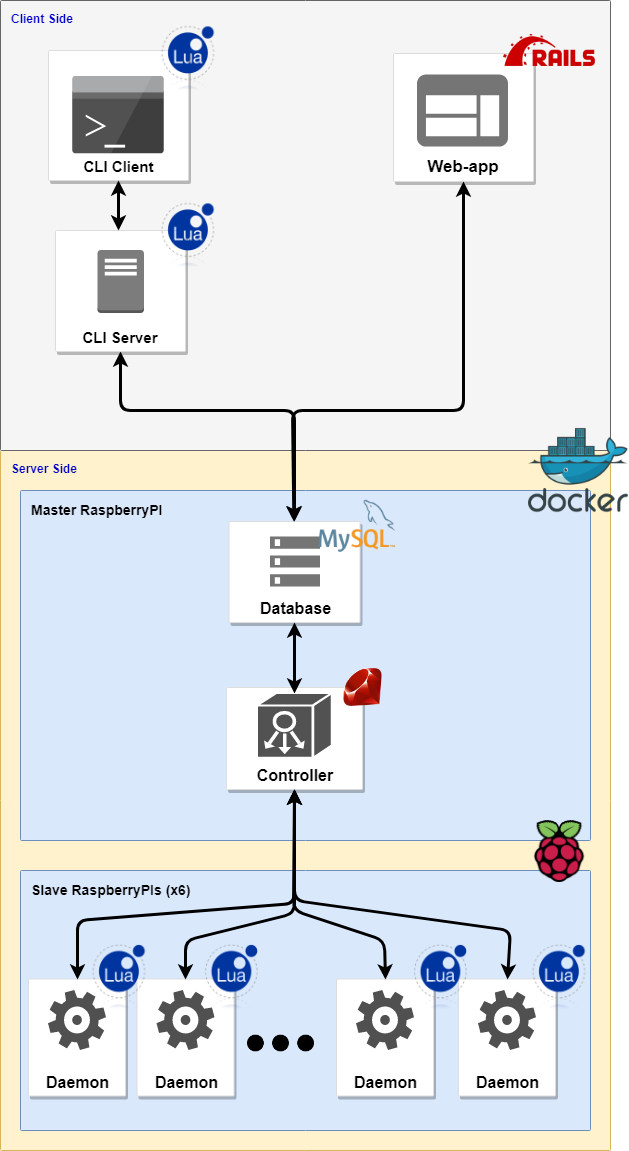
\includegraphics[scale=0.6]{figures/prev_arch.png}
          \caption{\label{prev_arch} Previous Splay Architecture}
        \end{figure}

        Whether through the usage of the CLI application or the web application,
        the user was able to interact with the Splay system and to send his
        jobs, and gather many informations such as the logs or the current
        state of the running Splayds (the Splay daemons).

        The fact that the database was the central piece of communication
        between the controller and the user applications was a design choice
        that we decided to respect and to keep working that way. Indeed, the
        \textbf{Controller} is the central piece within the Splay project,
        trying to push changes in that design choice and try to implement a
        different way of communication than the database would have, more
        than probably, implied a total rewrite of the controller.\\

        That being said, we weren't totally satisfied about the interaction
        possibilities offered to the user. Indeed, the Ruby on Rails application
        was quite old, and the client/server pair of the command line interface
        stack had a hard to maintain and to huge codebase compared to the
        features that it had to offer.\\

        We thus chose to operate major changes on this part of the Splay
        project, in order to combine the arrival of our new features and
        changes onto the core of Splay with a better user experience.

      \subsection{Renewed Architecture}

        The main issue on the architecture of the user services was a code
        duplication issue, or at least a duplication related to the solutions
        created to resolve a common problem. The Rails web application and the
        CLI server had the common role of letting the use manipulate the
        database to transmit and gather informations to the \textbf{Controller}.\\

        The first decision to make in order to solve this problem was to
        merge those two services into a single one and to call that new
        service according his role among the system: the \textbf{backend},
        according to the viewpoint of the client.\\
        This backend would have the ambition to offer a secured API through
        the usage of JWT \cite{JWT} and therefore allowing the development
        of services around that backend, in our case a web application and
        a command line interface application.\\

        The web application would thus use a recent JavaScript technology
        allowing dynamic interactions with the user, and the CLI would use
        a simple and dedicated technology, those two services consuming the
        same API offered by the backend. The backend, for its part, would
        stay in the Ruby ecosystem, in order to keep a technology concistency
        with the global project and the technologies already in use.\\

        The resulting reworked architecture would therefore be the following :

        \begin{itemize}
          \item The \textbf{Controller} : The core part of Splay, waits for jobs
          and dispatch them to the daemons.
          \item \textbf{Daemons} : Workers registering to the controller and waiting
          for jobs to achieve.
          \item A \textbf{MySQL DB} : The communication piece of Splay, allowing
          communication between the user and the system.
          \item \textbf{Backend} : The backend of the client side Splay app
          \item A \textbf{Web-app} : The single-page application
          \item A \textbf{CLI} : The command-line interface
        \end{itemize}

        \begin{figure}[H]
          \centering
          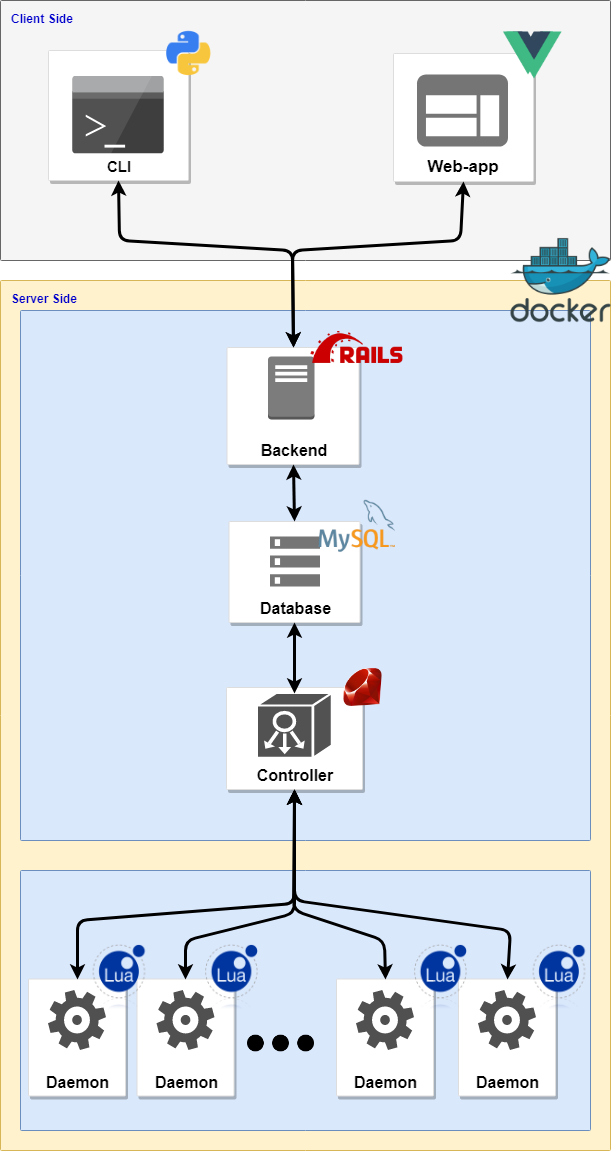
\includegraphics[scale=0.125]{figures/new_arch.png}
          \caption{\label{new_arch} New Splay Architecture}
        \end{figure}

    \section{Hardware Architecture}

      About the Rasp cluster. {\color{red} TODO}

  \chapter{Development Methodology}

    % Merge with test, global quality assurance chapter

    Before speaking about the implementation details, it may be useful to
    describe the way we organized ourselves in order to develop the application.
    The fact of being two student on this development project necessarily
    implied a way of organizing ourselves a bit more serious than a
    development project alone.\\

    Thanks to the courses about AGILE methodologies we followed during our
    scholarship, and the both of us having had the occasion of acquiring
    experience in a professional way through internships and part-time jobs,
    we wanted to put to work this knowledge and good practices acquired in
    the project management domain.\\

      \section{Kanban}

        The first tool we put in place, and this from the very beginning of
        the update period of Splay about which we talked in the previous
        sections, was a Kanban using the online website Trello \cite{trello}.
        The kanban allowed us to : \\

        Le premier outil que nous avons mis en place, et ce dès notre période
        d'update de Splay dont nous avons parlé plus tôt, a été un Kanban en
        utilisant le site en ligne Trello. Le kanban nous a permis de : \\

        \begin{itemize}
          \item Have a clear and precise view about the remaining tasks we had
          to achieve in the backlog, and also about the development state of
          all the other tasks.
          \item Encourage and even oblige ourselves to translate the features
          we had to implement into sufficiently detailed and explicit cards on
          the kanban. This process has the benefit of refining or making
          features the most explicit possible before starting the development.
          \item Have a way of tracking the project's progression and offering
          to all the people related to the project a simple and effective way
          to keep themselves informed about Splay's state.
          \item To focus ourselves on specific tasks and to work in an
          iterative and efficient way.
        \end{itemize}

      \section{Quality Assurance}

        This will be explained more explicitly in the next chapter, but we
        wanted to be sure that we would be able to keep a certain degree of
        quality in our work on Splay and more specifically at the code level,
        in order to ensure the overall maintainability of the project. We
        therefore set this goal through the setup of the following elements :\\

        \begin{itemize}
          \item \textbf{Testing suites} : Set of unit tests and integration
          tests, intra-services and inter-services.
          \item \textbf{Linter} : Static analysis of the code in order to
          satisfy to a set of rules about codestyle and good practices.
          \item \textbf{Coverage Analyzers} : Analysis of the percentage of
          the code coverage by the test suites.
        \end{itemize}

      \section{Github and Gitflow}

        The project and all the services composing it are versioned using the
        \textit{Git} versioning system and are hosted on the online service
        \textit{Github}.\\
        We therefore organized our work on the Gitflow model. Each feature or
        tasks we created on the kanban was meant to receive its very own
        branch, starting from the main branch.
        Once the feature finished and tested, a pull request was made asking
        to merge the feature branch with the main branch.
        The first benefit of this was obviously to keep the main branch in
        a working state with healthy and finished features.\\

        The second benefit of this way of working on the project was to
        permit, once again towards the goal of ensuring quality, code reviewing.
        Each time one of us was done with the development of a task and was
        issuing a pull request, the other was assigned as code reviewer and
        was in charge of making this code review, accepting the pull request and
        doing the merge, or to detect errors or bugs as the outcome of the
        code review and therefore to ask for changes to the pull request issuer. \\
        Besides the main code review's benefit of reducing the number of errors
        or bugs, this process also allowed each of us to keep itself aware and
        keep itself up to date with all the different changes happening on the
        different services. Indeed, it was impossible for us to work together
        in the mean time on each single service, because of the number of
        services and inter-dependant features we had to develop.

  \chapter{Implementation}

    \begin{itemize}
      \item Implementation choices details
      \item Story-telling about the development phase itself
      \item Details about the implementation, about how Splay is working today.
    \end{itemize}

    \section{Technology choices}

      \subsection{VueJS - Web App}

        As we made the decision that the web application would only be a
        front-end application making use of a centralized backend offering
        a complete JSON API, we canted to use a front-end web development
        framework that would satisfy the following conditions : \\

        \begin{itemize}
          \item Light
          \item Ease of development and maintenance
          \item Access to numerous third-party libraries
          \item Popular enough to be ensure support over time
        \end{itemize}

        In order to develop a front-end application, the JavaScript ecosystem
        was an obvious choice, and we made a pre-selection among the most
        popular web framework on the market and recognized for their qualities:
        ReactJS, Angular and VueJS.\\
        We rapidly removed Angular from our list because we preferred the
        component-based UI development offered by the two other frameworks,
        which were lighter and avoiding to have to develop in the MVC style.
        Even if we both had a previous experience with React thanks to a
        Cloud Computing course at the UCLouvain, we decided to go for VueJS
        instead of React.\\

        The first major advantage of Vue is how light it is, we also took into
        account the fact that this technology was gaining in popularity for
        multiple years now to be today a huge player in the world of the web
        technologies. Moreover, as we took some time to develop a proof
        of concept application using Vue, we were totally satisfied with the
        simplicity of development that that framework was offering to the
        developers and allowed us to be totally confident into the fact
        that going for this technology would allow any further contributer
        of the Splay project to easily get in and participate to the
        development.\\
        Indeed, a Vue application is organized around single components, each
        having their own HTML template, their CSS style declarations and
        the associated JavaScript code. No other exotic language is required.\\
        The fac tthat the framework is in the JavaScript ecosystem and
        associated to the NPM package manager also allow to take advantage of
        numerous existing libraries, such as data visualisation libraries,
        testing libraries, etc... \\

        For all those reasons, Vue revealed itself the best choice for a
        web application, and also allowing us to develop with a something
        we liked and with recent technologies, besides providing an efficient
        solution to the conditions we needed for the technology.

      \subsection{Python - CLI}

        The old pair of services intented to compose the CLI service was
        written in LUA on the client side, and the CLI server was in Ruby. As
        the server's logic would be moved and merged into the \textbf{Backend}
        service, and as we wanted to keep a command line interfact application
        in order to run tests of the global project, we needed to reevaluate
        the relevance of the LUA usage for this application.\\

        It is more than probable that LUA was used for coherence reasons back
        in the days, and to avoid to scatter Splay around too much different
        technologies (although Ruby may have been used too instead of LUA).
        Still, maybe today this choice was not the most relevant for a CLI
        application. Indeed, our small client CLI had to be :

        \begin{itemize}
          \item Simple
          \item Concise
          \item Written in an easy-to-use language
          \item Having conveniant libraries allowing to create simple CLI apps
        \end{itemize}

        However, we inherited of an application scattered in multiples LUA
        files, each file representing a CLI command. We therefore had a huge
        source of code duplication, as each file was repeating the process
        of parsing the user arguments when the program was called, and also
        repeating the process of reaching the server through a HTTP library
        in LUA.\\
        Ruby was indeed a relevant option if we wanted to restrict the number
        of different technologies in use among the project, but Python was
        a better choice to write such a simple script as our CLI. Python has
        a lot of very conveniant libraries to treat HTTP calls and to
        manage and parse user arguments when creating a CLI application.

      \subsection{Ruby on Rails - Backend}

        The controller service and the old pair of services composing the CLI
        having been developed with the Ruby language, and the old web
        application having been developed with Ruby on Rails, it was obvious
        for us to stay within the Ruby ecosystem to create the new service
        that would become what we called the \textbf{Backend}. The technology
        we wanted to use for this development had to offer an efficient
        solution to the following issues :

        \begin{itemize}
          \item Allowing a simple interfacing with the MySQL database in order
          to ensure the communication with the controller, and therefore allow
          the submission of new jobs, the gathering of information about the
          Daemons, etc...
          \item Allow to develop and expose a JSON API alloing other front
          end services (web application and CLI) to make use of this API and
          interact with the Splay system.
          \item Offer a large choice of libraries for testing, data
          serialization using JSON, and other libraries solving the problems
          we talked about before.
        \end{itemize}

        The both of us already having a certain experience in using Ruby on
        Rails, and for the reasons of ecosystem consistency we talked about
        in the previous sections, we immediately agreed on using this
        framework for the backend. The fact of staying in the same language
        ecosystem would allow us to make sure that future contributers to
        the application would not have to play with too many technologies and
        therefore make the future evolution of Splay easier.\\
        It should also be noticed that, as we exposed it when talking about the
        changes in the renewed software architecture of Splay, the previous
        web application and the CLI server had a similar role although being
        specialized for different applications. However, the commom logic
        of these two Ruby services was already present, and a part of the
        work was therefore just the matter of isolating this common logic
        and making it better.\\

        Indeed Rails allow to easily develop, besides traditional MVC web
        applications, API only applications that doesn't contain all the stuff
        and complexity needed for presenting HTML views to the user and thus
        having a lighter and more concise codebases.\\
        The ActiveRecord \cite{activerecord} ORM shipped with the Rails
        applications is also a major advantage for this technology, allowing us
        to easily and efficiently manage the system's jobs and daemons.\\
        Finally, the availability of some libraries such as RSpec made for the
        testing (topic on which we'll talk more deeply in a dedicated chapter),
        Rubocop for the linter, or even the Netflix's fast\_jsonapi library for
        data serialization has definitely made Rails the right technology to
        choose for the Backend.

    \section{Development}

      This section details in a story-telling way all the different part
      of our work on the project, starting from the first big code cleaning/refactors
      and ending with our latest features on the application.\\

      The organization of the section doesn't reflect a strict timeline of
      our work but is organized by date of beginning. Indeed, some goals
      and features needed further improvement over time.

      \subsection{Github Repository Reorganization}

        From our first analysis during our part-time job period on the Splay
        project, we weren't satisfied about how it was maintained on Github so
        far. Our major concern were the following :

        \begin{itemize}
          \item Lack of version tagging to specify stable versions
          \item The code organisation was not good and it was hard to
          understand exactly where the different services were located,
          everything was more or less in the same source folder.
        \end{itemize}

        From our last experience we also realized that the project was really
        lacking of documentation in order to help and guide people interested
        in Splay to install and run it.\\

        We therefore started with forking the project in a personal repository,
        allowing us to perform complete reorganization of all the directories
        and files composing the project and adding some basic documentation.
        Each service was successfuly placed in a distinct directory while
        keeping the docker-compose file working.\\
        The project was cleaner, however, we felt that this wasn't enough
        and that we could achieve a better structure. The project is big and
        consisting of multiple services interacting with each other but
        not sharing any code. We therefore decided to create a new Github
        organization called \textbf{The Splay Project V2} in which we created
        a distinct repository for each service and one as the main repository
        of the project.\\

        The main repository called \textbf{Splay} contains all the other services
        through the submodule \cite{GitSubmodules} feature of git. These
        subrepositories representing the new architecture wanted :

        \begin{itemize}
          \item the cli (command line interface)
          \item the daemon (also called \textit{splayd} in the project)
          \item the backend (the merge of the cli\_server and the old web app backend)
          \item The controller
          \item The new web application
        \end{itemize}

        Each of these subrepositories is self-sufficient and contains a Dockerfile
        allowing the user to create the related container and to use and test
        the service alone, and therefore also has it's own documentation.\\

        For each master branch of these subrepositories, a link with Dockerhub
        has been made so that each push on master will trigger an automatic build
        of a docker image using the source and uploading it on the Dockerhub \cite{DockerHubGithub}.
        This was especially made to ease the integration testing using a
        continuous integration service, which would have to build every single
        image otherwise.\\

        Now the services were clearly and logically separated in their
        distinct repositories, it would be really easier for us to track
        the changes made in each service and would ease further improvement
        by Splay maintainers.

      \subsection{Stabilisation of Controller and daemon}
        {\color{red} TODO}
        \begin{itemize}
          \item Integrated work after 2011
          \item fix with sequel call in all controller
          \item update openssl daemon
          \item fix bugs controller and daemon
        \end{itemize}

      \subsection{Centralization of Splay's Backend}

        As said before in the technology choices section, one big thing
        we wanted to achieve was the merge of the old CLI server and
        the backend part from the full-stack old web application as those two
        services were basically achieving the same work and holding the
        same responsibilities.\\

        We started with a fresh Ruby on Rails application, passing the
        generator the \textit{--api} option so that we were provided with
        a clean and simple Rails app without all the front-end dedicated
        files, making it simpler and lighter.\\

        Before writing any line of code, the following tools were added
        to the project :

        \begin{itemize}
          \item \textbf{Rspec}: A performant and easy to use Ruby testing
          framework to be able to begin development following the test
          driven development approach.
          \item \textbf{Rubocop}: A static code analyzer (linter) to follow
          good codestyle conventions and avoid bad pattern right from the start.
          \item \textbf{Travis}
          \item \textbf{CodeCov} A test coverage tool to get further
          information on the test suite.
        \end{itemize}

        Now that the app was ready for development, the major features
        we wanted to provide were the one provided by the old CLI server and
        were the following :

        \begin{itemize}
          \item User and session management (creation, login)
          \item Job management (creation, deletion, listing, details)
          \item Daemon querrying (listing, details)
          \item Job logs querrying
        \end{itemize}

        Implementing those features would let us immediately reuse the old
        CLI client for testing purposes and would provide sufficient actions
        to start the development of the web application, which could unveil
        need for new endpoints on the backend to provide user with more
        actions in order to interact the system.\\

        \subsubsection{Models}

          The first phase of this centralized backend development was to
          put it in charge of the database and the way the data was handled.\\

          For this purpose, we progressively created database migrations
          for each model of the Splay system (jobs, daemons, users, etc...)
          with the right constraints on their fields.\\
          We reflected these constraints inside the generated Rails models to
          ensure that no corrupted data could be registered into the system,
          having a double check through the application and through the
          database schema.\\
          For each model created, we also wrote model tests to ensure those
          constraints were respected when creating a new model and trying
          to save it into the database.

        \subsubsection{User Registration}

          To achieve the registration of users, we simply used the
          well-known Devise \cite{devise} gem (gems are how ruby libraries are
          called) which provide out-of-the box an efficient and flexible
          authentication solution for Rails application.\\
          As we were to allow the authentication through a future JSON API,
          the most relevant part in using Devise was to make use of all
          the user registration process given by the gem, using good principles
          in terms of password hashing with salt to store them. We didn't
          have to reinvent the wheel about user registration.\\

          Moreover, for any further development or evolution of the application,
          we know that Devise also provides user management modules such as
          Omniauth support, account tracking, registration confirmation
          through emails, and many other listed on the gem webpage.\\

          Devise was therefore the best choice for our registration management,
          even for an API only Rails application.

        \subsubsection{User Authentication}

          As we mentioned it before, one of the best way to handle user
          authentication in JSON API applications is by using the JSON Web
          Tokens (JWT), following the industry standard from RFC7519.\\

          Upon successful registration or login on the Rails application, a
          JWT is returned to the calling application to provide it with a way
          to authenticate further request. This JWT holds encrypted
          information (with a secret key) such as the user id to allow the Rails
          app to identify to whom belongs the request. The fact that the token
          is generated in the backend with a secret key also means that the
          token cannot be altered or forged by a malicious application.\\

          To make this works, we had to begin the work on the API endpoints.
          Before starting to work on those endpoints, we agree that we would
          follow the principles of REST \cite{rest} for the API. Endpoints would
          represent entities with classic HTTP verbs to interact with them.\\

          Each endpoint inside our system is managed by the following stack :

          \begin{itemize}
            \item A route entry representing the entity. In this case,
            authentication is linked to the session entity and achieve through
            a POST method, as we want to create a new session.
            \item A controller method corresponding to the endpoint action.
            Here then, a Session controller exists, with a create method in
            which the password checking happens and a response is returned
            accordingly.
          \end{itemize}

          As we were in the objective of following good practices, we wanted
          to follow the \textit{"Fat models, skinny controllers"} principle.
          But instead of bloating our models with the needed inner logic for
          authentication, we created intermediate layers called services
          in Rails. Those services hold the needed logic to keep the controllers
          nice and clean. In the case of authentication the controller receives
          the request from the router, filled with user data, then delegates
          the task of password verification, token generation if succeeded,
          and just return the result in the response.\\

          The same process was also applied to manage registration through
          the API, as it needed the JWT layer to be in a working state.\\

          Finally we also wrote tests simulating request making use of our
          API, which we'll explain in more details in a dedicated chapter.
          Nevertheless, each test is testing the different behaviour of
          the endpoints, like registering with a bad email, logging in with
          a non-existant user, etc...

        \subsubsection{Splay Endpoints}

          From all the previous tasks on the backend, we now had all the
          necessary basis to create the other endpoints in order to let
          an authenticated user interact with Splay.\\

          Once again, we created an authentication service that would check
          the request's token to verify whether or not the user was valid or
          if he had the necessary rights to perform the requested action.\\

          The endpoints we created are the following :

          \begin{itemize}
            \item \textbf{Users} : Create, destroy, index (get the list of that
            ressource)
            \item \textbf{Sessions} : Create
            \item \textbf{Splayds} : Index
            \item \textbf{Jobs} : Index, show (get info on a specific entity
            of that ressource), destroy and create
            \item \textbf{Logs} : Show
          \end{itemize}

          The create methods required additional checks in corresponding
          services, to carefully create the entity in the database with
          the data sent with the request and make sure those data were
          satisfying the constraints.\\

        \subsubsection{Error Handling}

          In order to provide the best response to the applications
          communicating with the backend, we wanted to give response
          the right HTTP errors code in case of errors.\\

          Indeed a successful request is automatically answered with a 200
          status code by the Rails application by default.\\
          Rails has a really conveniant way to raise errors and catch them
          in the same or upper component on the call stack, we therefore
          made use of that tool to implement the following error manaegement
          strategy :

          \begin{itemize}
            \item Each Controller of our API inherit from a common file
            called \textit{ApplicationController}
            \item This ApplicationController holds a set of catchers (rescue
            in the Ruby language) to catch which errors could happen in our
            application :
              \begin{itemize}
                \item The entity that the user wants to create isn't valid, this
                means he sent bad parameters through the request
                \item The requested action is not authorized for this user
                \item The request is malformed (missing fields or badly forged
                request)
                \item The requested entity doesn't exist (for example a user
                wants to get the job details for a non existing job)
              \end{itemize}
            \item Then in any controller or service used by a controller, we
            can raise an error and associate an error message, which will be
            autmatically rescued at the root level and trigger a response with
            the right HTTP status code and the given error message.
          \end{itemize}

      \subsection{The new front-end application} %TODO: Review - Rewrite

        In this section, we will talk about the new modern web application.
        The developement story beginning by a complete refactor of all features
        and finished by the new features developed in the web application side.

        \subsubsection{Single Page Application - Old feature refactor}
        As the devolment of backend was begon (previous section), we started, in the same time, the
        developement of the Single Page Application in VueJS. After removing
        old files of the previous web site, we created a basic VueJS project
        (version 2.5.X at this time) with the home page and the bootstrap-vue
        package \cite{BootstrapVue}. \textbf{Bootstrap} \cite{Bootstrap} is a
        well know HTML, CSS, and JavaScript framework to create responsive and
        modern web interface. The full integration of bootstrap in a Vue
        project is done with the extension of bootstrap package, bootstrap-vue.
        For us, Bootstrap is like a Swiss knife to make a web page with minimun
        design and modernity. \\

        The next step was to build a register and login page for the user
        management. To manage different page in the same Vue project, we
        installed the Vue-Router package. It is a extension of Vue to navigate
        through different pages (url) on the single page app (no reload with
        the server), and the user can switch page as he was on a regular
        website (backward/forward page, historic, ...). It is commonly used in
        front end framework to give a better user experience. Then, we created
        a page for the user registering and connection, directly connected to
        the backend user API. For the json communication with the backend, we
        used axios \cite{axios}, a popular HTTP Javascript client. At the end
        of this version of the web application, the user can create his/her
        account and connect to it, and the token of authentification (token
        based authentification) will be save on the client browser (auto-login
        for the next visit). \\

        % job - splayd list and job form
        In order to get the same features as the legacy website, we created a
        monitor page, where important information is given with lists. Indeed,
        a list of splay daemon (create by controller) is retrieve from the
        backend and print with global information in a nice bootstrap table.
        Also, a second table, used for jobs (also via the backend service), is
        builded with general data. The user can choose to see more details on
        one splay daemon or a job via a button. Also, he can choose to kill a
        job through a red button, the controller will do the rest. Moreover, The creation of job is done
        with a simple form and it is automatically checked with vee-validate
        package \cite{VeeValidate} (also checked in the backend service, of
        course). Vee-validate is a small package solutionning the problem of
        manual checking of form by adding some propreties to inputs, and it
        makes our code more compact and less messy. At this step, we had
        almost all legacy feature (for the web application) but in much more
        nice way, with modern solution and maintenable code. Only the log
        download was missing at this point. \\
        {\color{red} TODO : Screen shot of monitor}

        % Log
        When the log API on the backend was enable, we readd this feature to the website with some
        improvements. When the job running or endend, the user can see the log (with a button next to details)
        of merge daemon log with time and daemon indication for each line of log. The user can choose to
        download as a text file (as before), copy to the clipboard or only verify the log in
        the website checking for any error. \\

        \subsubsection{The Lua editor}
        % Lua editor
        The backend was not ready for the log feature, then we worked on the Lua editor
        integration. The idea to build our-self entirely the editor was moved aside quickly,
        it will take too much time and it will be not evolutive. Then, we found a
        great package, named brace (a browserify version of Ace editor) \cite{Ace}. Ace
        can handle hundred type of programming language for the coloration, error handling and
        show line number. The integration of ace is the project was easy and light, Lua is
        colorize perfectly and a error is show when the syntax is wrong. But, there is not
        build-in auto-completion for Lua most likely because Lua is not very popular these days.
        It is possible to add our own completer in the ace edito, but it is a long task
        for few results, then we decided to move on.
        {\color{red} TODO : screen shot of Lua editor}

        \subsubsection{Topology creation}
        % SAM: Topology creation
        {\color{red} TODO + screen shot}

      \subsection{Rework of the CLI to use new Backend}

        All the Command line interface has been redone in Python more clearly and concise. {\color{red} TODO }

      \subsection{Fault injection}
        The fault injection (or crash point) is done on the daemon side. Indeed, we wanted
        to crash the code in middle of the execution tree, then, only the daemon can
        handle with presicion the crash. We choose to use domain specific language for
        crash management that the user can put in a Lua comment. During the execution of job, the first step
        is to parse the code and manage the execute of the crash point.

        \subsubsection{Domain Specific Language (DSL)}

        We specified a small DSL designed to be simple and flexible, for the user and for the parsing. This DSL need to
        be integrated to the Lua code without modificatation of this one, and trying to avoid crashing the
        daemon if the specification (by the user) of the crash is not correct. Also, the number of line between the
        source code and after the parsing (DSL) need to be the same for error message (to get the correct line number in the trace).
        For these reasons, a crash point need to be reprensented in \textbf{one line} and beginning by two comma (--) which
        indicate comment in Lua and to avoid interpretate user comments, we add the keyword \textit{CRASH POINT}.
        The crash append where the crash point is define, then it is possible to
        crash everywhere (thread, middle of function, etc). \\

        Secondly, a fault is defined by it type, by the moment it occurs and on which nodes it going to happend.
        These characteristics need to be on the DSL specification. First, we begon to integrate the affected (by crash) nodes choosed
        (can be several), in this purpose, the user adds, after the keyword \textit{CRASH POINT},
        the ids of nodes (separated by space). We separated these and the type of fault by adding a colon, the type
        of fault is defined by its name and a possible extend data (also separated by space). Again, we split the
        fault type and the moment definition by a colon. The moment definition (when occurs the crash) is a keyword, follows
        by additional data. Our final DSL looks like (The first line corresponds to one line of crash point):
        \begin{lstlisting}[style=MyBash]
-- CRASH POINT id_splayd [id_splayd [...]] : <TYPE> : <WHEN>
<TYPE> => STOP | RECOVERY <float>
<WHEN> => AFTER <int> | RANDOM <float>
        \end{lstlisting}
        For now, you can see, there are 2 types of crash and 2 way to define the moment of crash. A stop crash (STOP) means that
        the nodes will be dead forever. In opposite, when it is the recovery type (RECOVERY), the node will be crash but restart
        completely after x seconds (float number). Moreover there are 2 way to define when the code will crash. The ATFER keyword
        is the determinist way, after x pass (int number), the next passage the crash will happen. The non-determinist way is
        done with the RANDOM keyword, there is a x probability of crash (float number between 0 and 1) at each passage.
        Here some positive examples of crash points using our DSL :

        \begin{lstlisting}[style=MyLua]
-- Crash forever the node 1 and 2 at the 4th passage
-- in the code
-- CRASH POINT 1 2 : STOP : AFTER    3

-- At each time that the code (node 1) pass by this comment,
-- there is 0.0002 chance to crash the node 1
--CRASH POINT 1: STOP : RANDOM 0.0002

-- Crash immediately when the comment is encouter in
-- the node 1, but this node will recover after 2 sec
-- CRASH POINT 1: RECOVERY 2 : AFTER 0

-- Have one chance on two to crash at each pass for
-- the node 1, 2, 3, 4, 5. But recover immediately
-- CRASH POINT 1 2 3 4 5 :RECOVERY 0:RANDOM 0.5
          \end{lstlisting}

        Also, we add some negative examples (won't product any crash) :

        \begin{lstlisting}[style=MyLua]
-- Won't work because Crash point not in uppercase
--Crash Point 1 2 : STOP : AFTER 3

-- Won't work because no node is specified.
-- CRASH POINT :RECOVERY  965 :   AFTER 3

-- Won't work because RECOVER is not a valid
-- type (but warning expected).
-- CRASH POINT 1 2 :RECOVER 1 : AFTER 3

-- Won't work because TIME is not a valid type
-- for now (but error expected).
-- CRASH POINT 1 2 :RECOVERY 1 : TIME 3
        \end{lstlisting}

        \subsubsection{Parsing}

        The parsing of the code is done just before that the user code is launched in each node (daemon). The parsing will
        create a table with information of each crash found in the user code and concerned with this node (with id node).
        This table is save in the library named "splay.crash", and the access of crash information is done by a number id.
        The parsing will return a new code where the crash point comment take in account (if no error and concerned this node)
        is replaced by a function calling, with the right number crash id (as parameter). Then, when the code will execute,
        and the crash function call, we can act depending of information about this crash (type, when trigger the crash, ...).\\

        The parsing handles savely the error of user about the syntax, with crashing the node. Parsing is done
        line by line and if there is a error (also in the code of parsing itself), the line will be unchanged and
        a warning or error log will be written. Also, the parsing is fully write in Lua (of course) with only
        the regex (not standard regex) matcher of Lua \cite{RegexLua}.

        \subsubsection{Execution}

        Well, we see the definition of the DSL and how we parse it, now we will detail how the crash append and how
        to handle it to recover. First, the main problem is that Lua multithreading is non-preemptive, then we can't
        stop a thread from outside \cite{CoroutineLua}. The only to stop directly the Lua interpreter and kill all other
        thread is to exit the program by a os function. Also, we have the possibility to send a exit status code of the
        process, it is very convinent for knowing if we need to restart or not after a crash point. \\

        With this way to exit, we can create a artificial crash point, which kill immediately all coroutine (thread)
        of Lua and the current execution. Moreover, we can pass special exit status code to send message to a other process.
        To use this exit code, we created a fork (already in the c splay lib) before parse the crash point and execute the user code.
        Then the process child will execute the parsing of crash point and execute the code, and the parent process will wait
        to get the exit status code of it child process. We added a Lua function (waitpid) for this purpose and use the
        original waitpid of C \cite{waitpid}. \\

        When the child process end (either normaly or by a crash), the parent process check the status exit code and act depending.
        If it is the exit code 65 or 66, it means that a crash has been done (or the user want to exit with one of these values),
        65 means a STOP crash, then no restart need to be node. On the opposite, 66 (Recovery crash type) means than we need to
        relaunch the user code,
        and it is done recursively (with a new fork of course), and the crash table is reset (by reparsing the original code).

      \subsection{Timeline Animation of a graph evolution}
      % REM
      {\color{red} TODO}

  \chapter{Testing and Validation}

    In this chapter, we will talk more deeply about the way we wanted to ensure
    the testing and the validation part in the Splay project, whether it be
    at the global system level or at the user functionalities level, each
    section will go through the different services and how we tested it, and
    also how we tested the application globally.\\

    The fact that Splay had barely no tests at all in the state we receive it
    motivated us into developing a solid test suite for the system.
    Indeed that fact made our task much more harder because we were progressing
    in the dark, each minor change was prone to create dysfunctions that we
    might only notice way later during our work.\\

    The test writing phase took place during the whole architecture renewal
    phase described previously, to make sure that we were ensuring the new
    code's maintainability, but also to progressively gives Splay's core
    new tests to have a healthy and maintainable final product.

    \section{Testing in Web App}

      As we choosed Vue as our framework for the web application service,
      all we had to deal with was components. As Vue is organised around
      the use of components, the immediate reward of this was that we would
      be able to write tests dedicated to isolated and simple components.

      \subsection{Jest}

        In order to test the components composing the application, we
        went for the Jest \cite{jest} testing framework, which was advised
        as unit testing framework during the project creation.\\

        Testing JavaScript is not always the simplest thing to achieve, the
        ecosystem being in constant evolution with diverse solutions emerging
        trying to fit with the evolution and the apparition of a lot of
        other JavaScript framework.\\
        But Jest was a really good pick as testing framework, as it was
        developped by Facebook and designed to fit with the majority of the
        most used front-end framework and this with almost no configuration and
        providing us with a really simple API.\\

        In order to test the application using Jest, we created a directories
        hierarchy reflecting the Vue components hierarchy we created, thus
        a test file corresponding to a component file. In each of these
        test specifications, we decided to target the core part of each
        components : the methods.\\
        Indeed, there is no need to test whether or not a click on a button
        triggers the associated action as this is part of the Vue system. What
        we wanted to test was the triggered action we wrote ourselves and
        were simply functions.\\
        Each file therefore tests that the related components can be
        successfuly instanciated among the application, then run a serie
        of \textbf{unit tests} validating the methods expected behaviour.

      \subsection{ESLint}

        Provided almost by default when creating a new Vue project, ESLint
        \cite{eslint} is a JavaScript linter that allows the developper to
        make sure he's not writing code inducing problematic patterns or not
        respecting code guidelines.\\
        This helps to keep a consistent codestyle as we were two people working
        on this project, and increase the overall code quality and
        maintainability. We chose not to change any preset of the shipped-in
        ESLint confguration to ensure following common guidelines among the Vue
        community and make sure any developper joining the Splay project will
        be able to work on the web application seamlessly.


    \section{Testing in Backend}

      As a reminder, the Backend such as we conceived it has the following
      roles :

      \begin{itemize}
        \item It has the responsibility of handling the database and
        defining its structure.
        \item It must offer a JSON API allowing other application to interact
        with the system.
      \end{itemize}

      The backend being written in Rails, we therefore have access to the
      ActiveRecord ORM which allows manipulating the database by associating
      tables to models. These models are thus granted with attributes,
      constraints to comply with on these attributes following the constraints
      listed in the database schema, but also granted with methods. This data
      modelisation allow us to do model testing.

      The backend role being only to offer a JSON API to the different client
      services through an authentication system using JSON Web tokens, a
      request testing suite should be implemented to validate our set of
      endpoints and the mechanism of authentication.
      The data responses being sent to the calling applications under the form
      of JSON responses, we had to serialize our models and therefore this
      part was also subject to testing.

      \subsection{RSpec}

        RSpec \cite{rspec} is a library aiming to ease Behaviour Driven
        Development on Ruby projects. BDD and TDD (Test Driven Development) are
        practices we wantedto follow for our work on the Splay development,
        this would allow us to adopt a green-red-refactor work cycles but also
        to focus on writing natural language scenarios and then translating
        them into test scenarios.

        \subsubsection{Model Testing}

          As we made it explicit in upper sections, the Rails ORM layer offers
          a reflexion about the database constraints by representing its
          tables under the form of models granted with attributes, that we can
          enrich with additional attributes, methods and an overlay of
          additional validations (such as validations on attributes
          combinations, or more complex constraints between the models).\\

          This additional abstraction therefore needs to be covered with a
          sufficient validation set, which we did by applying
          \textbf{Model Testing}, challenging that overlay applied to the
          models but also the basic constraints explicited in the database's
          schema.\\

          This testing set is therefore offering a double validation on the
          database field constraints, but also validations on the business
          logic we added in the application.

        \subsubsection{Request Testing}

          The request tests inside the Backend service are the most important
          tests we wrote, in terms or code coverage but also in terms of
          testing the implemented features inside of this Splay service.\\

          The request specs among the RSpec tool are made to simulate
          the behaviour of a third-party application sending a request to
          our service and therefore making the whole Rails stack running
          to provide an answer to this request.\\
          Each request is therefore going through those elements :\\

          \begin{figure}[H]
            \centering
            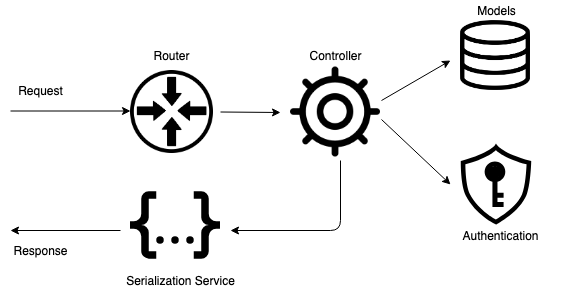
\includegraphics[scale=0.6]{figures/request_test.png}
            \caption{\label{request_test} Request Lifetime in Backend Service}
          \end{figure}

          Each route of the application is tested, exploring different possible
          scenarios for the incoming request (the idenfication token provided
          is invalid, the token is valid but the requested action is not
          authorized for the associated user). We therefore have a testing set
          that uses the whole application, simply by sending request and
          making expectations about the awaited response from the application.

      \subsection{Code Coverage - Simple Cov}

        We chose to use Simple Cov in combination of the testing applied to
        the Backend. This tool allow to measure the code coverage of Ruby
        application and to provide the developer with useful information
        thanks to its test execution analysis.\\

        Our ambition on the user part of the Splay project was a total recast of
        the services in more simple and maintainable ones, it was therefore
        obvious and simple for us to reach a total coverage of that new codebase
        with a test suite, and thus chose to use that tool.

      \subsection{Code Quality - Rubocop}

        we used Rubocop as the last piece of the tool stack designed to ensure
        the code quality within the service. Rubocop is a static code analysis
        tool (linter) allowing to detect violations to a set of rules about
        the code style and good practices (too many lines of code for a method,
        to many variables instanciations, too many conditional branching
        in the code, ...).

    \section{Testing in Daemons}

      The daemon is a critical part of the project, it allows the communication, the running
      and controlling the status of jobs. But the daemon also serves the user with a rich Lua Splay library.
      In the legacy project very few tests has be made to check the installation and
      test some very basic features (small functionalities) of the Lua Splay library. Also some tests didn't pass anymore
      (if there did passed one day?), and there was no testing library used. \\

      We wanted to improve this condition, we added a test library called busted \cite{busted}, it was the more elegant,
      active library and fully integrated with Lua 5.3. Then, we tranformed the old successfuly manual tests into busted tests.
      Only with this change, we detected some anomally in the lib code and fixed it. We added a test step in the
      docker creation to avoid the creation of malformed images (Unfortunately the docker becomes less compact and clean). \\

      Moreover, we added a lot of tests about all modifications (openssl updated, new misc functions, small change in existing functions, ...)
      and the new fault injection feature (parsing, crash and waitpid+fork). Sadly all the Splay lib, isn't tested, and far away from it,
      the huge amount of code (some not documented/used) make impossible to do it ourself. But, we ensure that our job is
      maintainable for future improvement/refactor.

    \section{Integration Testing}

      In order to automatically test the project as a whole, we also wanted to
      develop a functional test suite. This test suite would be relatively
      simple but complete enough to make sure that we could test the developed
      features in a global way among the system, and to achieve this goal we
      just had to translate our user scenarios into test scenarios.\\

      For these functional tests, we didn't use a complex technology and
      thought that a Bash scripts serie would be more than sufficient to
      reach our goal. Bash scripts could indeed not allow us to recreate user
      behaviour using Splay through the web application, but as this
      application is using the exact same API offered by the Backend than the
      CLI application, we could simulate user behaviour through that CLI (and
      that's partially the reason why the decided to keep a CLI application
      within the project).\\

      The integration tests were placed in a dedicated directory at the Splay
      project's root, and execute the following actions for each test :

      \begin{itemize}
        \item Cleaning the containers.
        \item Rebuilding the different services listed in the docker-compose
        file.
        \item Starting up the services.
        \item Executing commands through the CLI.
        \item Checking the returned responsed sent by the CLI and displaying
        whether the test phase has succeeded or failed in the terminal.
      \end{itemize}

      {\color{red} Link with scenarios}\\

      By proceeding this way and with the fact of using our user scenarios to
      determine the actions described in the test suite, we can make sure
      that the implementation of our features is functional and will stay
      functional through the lifetime and evolutions of Splay. Moreover, those
      tests are adding an additional validation layer compared to the tests
      targeting the different services individually. We have here tests that
      are involving each service in concrete scenarios and reflecting real
      working conditions of the project, and also testing interactions
      between the services.

    \section{Continuous Integration}

      Once again in a way to ensure quality, the different services were placed
      on the Travis CI \cite{travis} continuous integration platform. Travis
      can be coupled with Github to detect any change on the branches and
      automatically run a test procedure listed in a script and then offer
      feedback on how the test suite went.\\

      Splay being an open source project, that we hope to see growing in the
      future, its collaborative development will inevitably happen through
      the Github organization in which the different repositories are located.\\
      The coupling of Travis with Github allow, in the case of a pull request,
      gather the review about the test execution on the branch asking to be
      merged with the main branch, and therefore to make sure the build is
      clean and the test are passing before merging the new code.

    \section{Overall Testing Suite}

      Here is a figure detailing the whole Splay project with the different
      test suites and procedures that have been described in the previous
      sections so that the reader can get the grasp on the overall
      organisation of this.

      \begin{figure}[H]
        \centering
        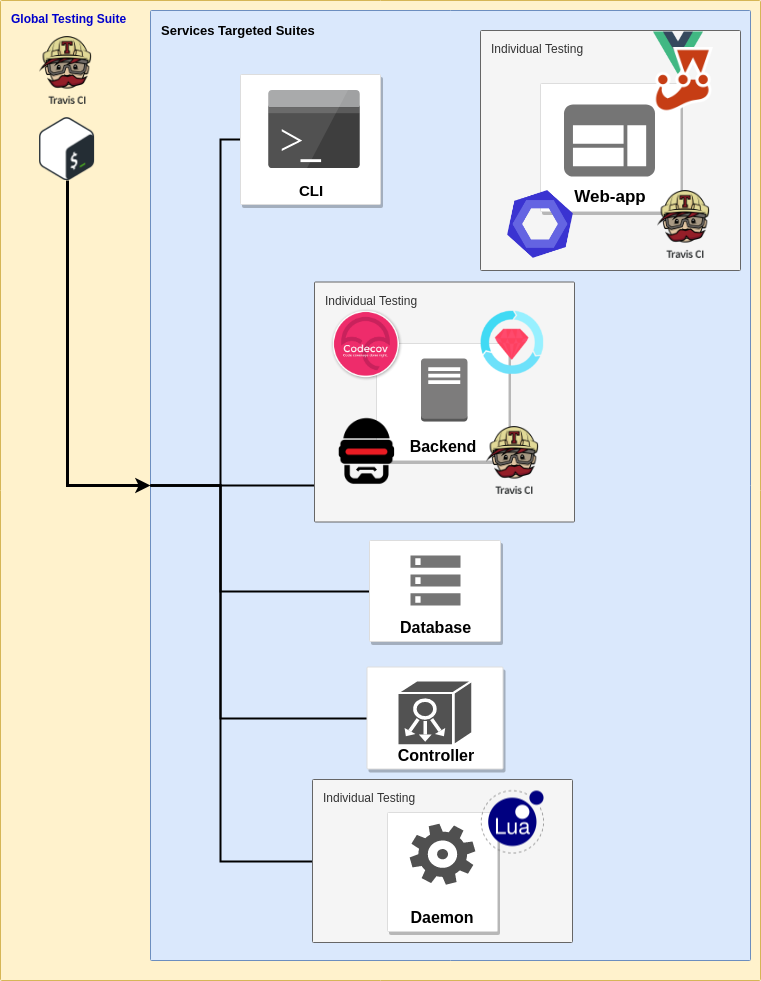
\includegraphics[scale=0.6]{figures/global_testing.png}
        \caption{\label{global_testing} Global Testing in Splay}
      \end{figure}

  \chapter{Use Case}
    A student following a course on distributed application wants to try raft (focus on the correctness of the leader election)
    implementation on 5 nodes.
    He choosed to use Splay for his tests in his own laptop (or cluster of mini-computer) but there
    is no installation of Splay available for him.
    We going to described the different step of this student with the usage of Splay.

    \section{Installation of Splay}
      First this student need to get a clean installation of Splay. Fortunately, this work is greatly
      helped because of a installation documentation and the dockerization of the project.
      Following the main README file of the main repository (production installation), he installs docker and
      docker-compose first. Then for running Splay, he runs the requested (by the README) commands in his terminal :
      \begin{lstlisting}[style=MyBash]
docker-compose -f docker-compose.prod.yml up -d web_app controller
# 7 daemons because it is recommended to have more than needed
docker-compose -f docker-compose.prod.yml up -d --scale daemon=7
      \end{lstlisting}
      Then he access to the web application of Splay with his favorite modern browser (not lynx, please) with this url :
      \url{http://localhost:8080/}. He creates is own account by the register form and it will be automatically connect next time.

    \section{Implementation of Raft in Lua}
      After the successful installation, the hard work need to be done, it means to create the implementation of raft
      with the help of the Splay library. Raft is not a trivial algorithm, but a understandable one.
      We based our algorithm on some papers \cite{RaftPaper} and articles/courses \cite{RaftSlide} \cite{RaftSite}.
      We have done the Lua code of the leader election of raft consensus helped with the Splay lib \cite{SplayLib}. \\

      \subsection{Creation of the algorithm}
      We will explain the raft election in small piece with each time the Lua code attached to it.


      \subsection{First result}
      % After doing the code of raft, he wants to try on several nodes (5), beginning without network topology (all nodes is directly connect).

      % He sees the log to check if one node is leader and no more.
    \section{Topology settings}

      % After checking his previous code, he repeats all process with and network topology.
    {\color{red} TODO}

    \section{Robustness Test through fault injection}

    % He wants to test the correctness of his code by making crash the leader essentialy, but also the other.

    {\color{red} TODO}

    \section{Result with a animation}
    % For any case, he wants to see the evolution of the nodes graph during the execution by parsing the log.
    {\color{red} TODO}

  \chapter{Improvements}

    % Our features
    \section{Our possible Features improvement}

      \subsection{Lua editor}
      {\color{red} TODO}
      \begin{itemize}
        \item auto-completion
        \item color theme option to choose
        \item integration of the splay lib to the auto-completion
      \end{itemize}

      \subsection{Crash point}
      {\color{red} TODO}
      \begin{itemize}
        \item new type of crash point (network crash)
        \item new type of when the crash append
      \end{itemize}

      \subsection{Topology Creation}
      {\color{red} TODO}
      \begin{itemize}
        \item automatic completion of edge between nodes
        \item modification of edge or nodes on double-click (modal)
      \end{itemize}

    % From old project
    \section{Security issues}
    {\color{red} TODO}

    \section{Refactor of Controller/Daemon}
    {\color{red} TODO}

  \chapter{Conclusion}

    \section{Objectives achievement}

    \section{Go futher}

  \nocite{*}
  \bibliographystyle{plain}
  \bibliography{biblio.bib}

  % Back cover page
  \backcoverpage

\end{document}
